% https://tex.stackexchange.com/questions/144577/remove-chapter-number-from-bibliography

\documentclass[
a4paper, 
11pt, 
ngerman,
listof=totoc,
%oneside,
%bibliography=totoc,
bibliography=totocnumbered,
abstracton
]{scrreprt}

\usepackage[T1]{fontenc}
\usepackage[utf8]{inputenc}
\usepackage[ngerman]{babel}
\usepackage{graphicx}
\usepackage{lipsum}
\usepackage{csquotes}
\usepackage[onehalfspacing]{setspace}
\usepackage{scrlayer-scrpage}
\chead*{\pagemark}
\cofoot*{}

%\usepackage{lineno}
%\usepackage{layout}
%
%\makeatletter
%\renewcommand*{\lay@value}[2]{%
%	\strip@pt\dimexpr0.351459\dimexpr\csname#2\endcsname\relax\relax mm%
%}
%\makeatother

%\usepackage[showframe]{geometry}
%
%\geometry{
%	top = 2.5cm,
%	bottom = 2.5cm,
%	left = 3.5cm,
%	right = 2.5cm
%	}

\usepackage[
backend=biber,
style=authoryear-ibid,
%sorting=ynt
]{biblatex}
\addbibresource{gravitropismus-bibliography.bib}

\title{Untersuchung von Gravitropismus bei \emph{Lepidium sativum} mit einem selbstgebautem Klinostat unter Zimmerbedingungen}

\subtitle{W-Seminararbeit im Fach Biologie am Luitpold-Gymnasium München}

\author{Alexandra Smirnova}


\begin{document}
	
\begingroup
\renewcommand*{\chapterpagestyle}{empty}
\pagestyle{empty}
\maketitle
\tableofcontents
\clearpage
\endgroup
	
\renewcommand\abstractname{Abstract}
\begin{abstract}

[Seit 1806 weiß man, dass Pflanzen sich an der Schwerkraft orientieren (Knight,1806). Dabei wachsen die Organe wie zum Beispiel der Spross nach oben, um Photosynthese betreiben zu können, während andere Organe wie beispielsweise die Wurzel nach unten wachsen, um Wasser und Mineralionen aufnehmen zu können.

Zum einem ermöglicht es den Pflanzen, um die begrenzten verfügbaren Ressourcen zu konkurrieren, zum anderen sorgt diese Fähigkeit dafür, dass die Pflanzensprossen nach dem Regen oder Windaktion jeglicher Art sich wieder aufrichten können. 

Außerdem können Pflanzen mit dieser Bewegungsorientierung ihre Samen von Bodenfeuchtigkeit und Krankheitserregern fernhalten. (Gravitropism in higher plants)]



[Gravitropismus umfasst mehrere Schritte, die in einem spezifischen Antwortweg organisiert sind.

Dazu gehört die Wahrnehmung eines gravistimulus (Reorientierung im Schwerefeld), die Übertragung dieses mechanischen Reizes in eine physiologische cal-Signal, die Übertragung dieses Signals von der Stelle der Erfassung an die Stelle der Antwort und eine Krümmung-Antwort, was es der Organspitze ermöglicht, das Wachstum in einem vordefinierten Einstellwinkel vom Schwerkraftvektor wieder aufzunehmen.

Die primären Stellen für die Gravitationserfassung befinden sich in der Kappe für Wurzeln und in der Endodermis für Triebe.

Die Krümmungsantwort tritt in den Dehnungszonen für jedes Organ auf.

Nach der Gravistimulation scheint ein Auxin-Gradient über das stimulierte Organ hinweg erzeugt zu werden und an die Stelle der Reaktion zu übertragen, wo es eine differentielle Wachstumsreaktion fördert.

Während also der gravitationsinduzierte Auxin-Gradient von der Kappe zu den Elongationszonen in Wurzeln übertragen werden muss, besteht kein Bedarf an einem longitudinalen Transport in Sprossen, als Stellen für die Gravitationserfassung und
Antwortüberlappung in diesem Organ.
(thaliana: A Model for the Study of Root and Shoot Gravitropism)]
	
	
\end{abstract}

% \let\raggedsection\centering
% \section*{\abstractname}
% Dies ist die Zusammenfassung auf Deutsch.

\chapter{Gravitropismus als wichtige Pflanzeneigenschaft}
	
\chapter{Fachliche Analyse der Thematik: Gravitropismus}

\section{Gravitropismus}

Die Bestimmung der Wachstumrichtung der Wurzel und des Sprosses unter dem Einfluss der Schwerkraft wird als Gravitropismus (Geotropismus) bezeichnet.

Dabei werden drei Bewegungen unterschieden: Positiv gravitrop, negativ gravitrop und transversalgravitrop.

Positiv gravitrop bedeutet, dass das Wachstum zur Schwerkraftquelle hin (nach unten) erfolgt.
Positiv gravitrope Organe wären zum Beispiel Wurzeln, Rhizoide (wurzelähnliche Strukturen), Moose oder Farnprothallien.

Negativ gravitrop dagegen bedeutet, dass die Organe wie Sprossen, Sporangienträger der Schimmelpilze der Gattung \emph{Mucor} oder Fruchtkörper mancher Pilze von der Schwerkraftquelle weg (nach oben) wachsen.

Diese beide Wachstumsrichtungen werden auch als Orthogravitropismus bezeichnet, da sie beide parallel zur Schwerkraft hinwachsen \parencite[546]{Jacob}.

Seitenwurzeln der ersten Ordnung (Nebenwurzeln, die von der Hauptwurzel entspringen) und zahlreiche Seitenzweige sowie Blätter wachsen transversalgravitrop: entweder flach oder quer nach unten in einem bestimmten Winkel \parencite[449]{Strasburger}. 

Legt man eine Pflanze quer, so werden sich die Organe, Wurzeln und Spross, krümmen, bis sie senkrecht stehen und wieder positiv bzw. negativ gravitrop wachsen
\parencite[528]{Luettge}.

\section{Differenzielles Wachstum}

Die Krümmungsbewegung wird meistens durch differentielles Wachstum zweier Organhälften, deren Bereiche wachstumsfähig sind, hervorgerufen.
Die Krümmung bei einer quer gelegten und gravitrop reagierender Pflanze wird hinter der Spitze der Hauptwachstumszonen der Wurzeln bzw. des Sprosses verlaufen. Andere Teile bleiben dabei ungekrümmt.

Bei Wurzeln ist die Streckungszone kurz, deswegen ist der Krümmungsverlauf relativ einfach. Bei Sprossen dagegen beginnt die Krümmung zuerst an der Spitze und dann immer weiter basalwärts fort, wobei der Spross sich gravitrop über die Lotrechte hinaus aufkrümmt.
Daraufhin findet eine Rückkrümmung statt, bis der Spross, nach einigen Pendelbewegungen, wieder senkrecht steht.

Diese Pendelbewegungen, die teilweise nicht von der Erdanziehungskraft abhängen, entstehen, wenn die Pflanze sich zu sehr überkrümmt, wodurch neue gravitrope Reize verursacht werden \parencite[450f]{Strasburger}.

Damit es zur einer Krümmung kommt, werden zuvor Reize durch Statolithen, schwere Körperteilchen oder Organelle in bestimmten Zellen des Sprosses, der Koleoptil-,und der Wurzelspitzen, aufgenommen. Es handelt sich dabei meist um Amyloplasten, die aus Stärke bestehen \parencite[530]{Luettge}.

Jedoch entscheidend ist der Stärkegehalt  der Amyloplasten, denn ohne ihn geht die gravitrope Reaktionfähigkeit verloren, so als würde man die Wurzelhaube entfernen, wobei das Längenwachstum der Wurzeln weiterhin unbeeinflusst bleibt.

Die Stärke aus den Statolithen-Amyloplasten kann man durch experimentelle Eingriffe, zum Beispiel durch Kühlung, verschwinden lassen \parencite[452]{Strasburger}.

Amyloplasten sind in Statocysten, Zellen, die Graviperzeption befähigt sind, zahlreich vorhanden und bilden meist ein Gewebe, die Statenchyme, wenn sie in großen Mengen vorkommen. Diese Stärke enthaltenden Bereiche findet man bei den Wurzelhauben und bei Stärkescheiden der Sprossachsen.  

Statolithen üben einen Druck auf Gravisensoren aus, wenn sie von der Schwerkraft beeinflusst werden. Wird die Lage der Pflanzen und ihrer Zellen verändert, so führt dies zu einer Änderung der Druckwirkung, wodurch die Graviperzeption ermöglicht wird \parencite[501f]{Nultsch}.

Diese Gravisensoren sind "Polster" von Membranen des endoplasmatischen Retikulums (ER), auf denen die Statolithen ruhen.
Dabei haben die Statocysten, in denen sich Amyloplasten befinden, eine zu den angeordneten ER-Polstern anpassende Form, sodass bei einer Drehung (aus der senkrechten Lage) der Statolithendruck auf das ER der Statocysten auf einer Seite momentan aufgehoben wird: auf der linken Seite bei einer Rechtsdrehung, auf der rechten Seite bei einer Linksdrehung.

Dadurch erfolgt die Graviperzeption schneller, denn die Verlagerung der Wurzel hängt  mit der Aufhebung des Statolithendruckes auf die ER-Polster links oder rechts der Wurzelhaube zusammen. 

Das von der Graviperzeption entstandene Signal kann nur in der Streckungszone hinter der Wurzelspitze aufgenommen werden. Kommt das Signal an, so setzt die Krümmungsbewegung ein, in dem die Flanken anfangen ungleich zu wachsen. Damit ist feststellbar, dass der Perzeptions- und Reaktionsort getrennt sind.

Für diese Reaktion sind Präsentationszeiten des Reizes wichtig. Sie liegen meist zwischen 2 und 85 Minuten. Das dauert viel länger, als die kürzesten Reizeinwirkungen, die unter 30 Sekunden liegen und noch wahrgenommen werden können.

Somit wird bei jeder kleinen und kurzen Reizeinwirkung eine Vollführung der Krümmungsbewegung vermieden. Das ist wichtig für Pflanzen, um zum Beispiel nicht bei jedem Windwehen unnötigerweise  sich krümmen zu müssen \parencite[531]{Luettge}.  

Die danach folgende Signalübermittlung durch den direkten Kontakt zwischen den Amyloplasten und ER wird als gravisensorische Transduktion bezeichnet.
Durch den Druck der Amyloplasten auf die ER-Membranen wird ein [Ca2+]-Efflux (das Austreten von Molekülen oder Ionen an der Zellmembran) aus dem ER verursacht.

Dadurch wird die lokale Calcium-Konzentration im Cytoplasma (flüssige "Grundsubstanz" innerhalb der Zellmembran) erhöht. 
Es wurde aber durch Untersuchungen an anderen Pflanzen festgestellt, dass der Druck auf eine einzige ER-Zysterne ausreicht, um einen Efflux zu verursachen.

Wichtiger bei der Signalumwandlung sind jedoch die Änderungen des elektrischen Feldes, die die Wurzel umgeben.
Bei senkrecht stehenden Pflanzen wandern ständig positive geladene Ionen (hier: Protonen) in die Wurzelspitze ein und treten im Bereich der Zellstreckzone wieder aus.

Diese Ionenbewegung wird als apoplastischer Strom bezeichnet, der ein elektrisches Feld, das die Wurzel umgibt, erzeugt. Dieses Feld ist mit einer hochempfindlichen Vibrationselektrode nachweisbar. 

Wird nun die Pflanze horizontal gelegt, so werden die Wurzeln gravitropisch gereizt. Dabei gelangen die Protonen nur noch in die untere Flanke der Wurzelspitze hinein und auf der Oberseite hinaus, wodurch auch das elektrische Feld sich ändert.
Jedoch die These, dass bioelektrische Phänomene sich an der gravitropischen Transduktion beteiligen, kann nicht verallgemeinert werden.

Die Ursache, der darauf folgender gravitropischer Krümmung bei Sprossachsen und Koleoptile, ist die durch Schwerkraft hervorgerufene asymmetrische Verteilung des Hormons Auxin (dies wurde bei verschiedenen Pflanzen nachgewiesen worden).

Auxin spiel aber bei manchen Pflanzenarten (z.B bei Sonnenblumen \emph{Helianthus}  oder Bohnen \emph{Phaseolus}) eine untergeordnete Rolle.
Die Steuerung der Krümmungsbewegung dieser Arten übernehmen dann Gibberlline (ein weiterer Pflanzenhormon) \parencite[502f]{Nultsch}.
  
Dies ist aber nur der Fall bei Organen höherer Pflanzen, denn bei einer Einzelzelle, beispielsweise werden die \emph{Chara} -Rhizoiden genommen, erfolgt die Streckung nur durch Spitzenwachstum (einseitiges Wachstum der Zelle).

Dictyosomen (flache, membranumhüllte Hohlräumen in der Zelle) synthetisieren dabei Membran- und Zellwandbausteine unter dem Bereich der wachsenden Spitze und transportieren dorthin die entstandenen Vesikeln (runde Bläschen).
Sie bevorzugen auf der Oberseite zu wandern, da beim Verlagern der Statolithen auf die Unterseite, der Weg dort damit gesperrt wird. Bei der Oberseite bewirken sie somit ein verstärktes Wandwachstum, also einen positiven Gravitropismus.

Bei gravitrop reagierenden Pilzen werden Amyloplasten durch "Glanzkörper" ersetzt, die die Funktion der Statolithen übernehmen, da Pilze keine Stärke enthalten. Diese in speziellen Vacuole liegenden Einschlusskörper besitzen einen hohen spezifischen Gewicht, da sie aus [BaSO4] bestehen.

Bei mehrzelligen Pflanzen (z.B. Bäume) wird  nach der Graviperzeption und in der darauf folgender Kette der gravitropen Reaktionsfolge  das Auxin, genauer gesagt das IAA (Indolessigsäure) in der physikalischer Unterseite der Sprossachsen sowie Wurzeln in höherer Konzentration aufgefunden.

Auf der Seite erhöhten oder erniedrigten IAA-Gehalts wird dann bei Stämmen das Reaktionsholz gebildet.
Wegen der Hemmung des basipetalen (abwärts strebend) Auxinlängsttransport auf der Oberseite, die die Schwerkraft hervorruft, wird ein seitlicher Auxintransport zur physikalischer Unterseite verursacht. Es wird dabei berücksichtigt, dass [Ca2+]-Ionen bei den beiden Prozessen beteiligt waren.

Dadurch verstärkt sich das Wachstum in der Unterseite, die sich dadurch anfängt zu runden, wodurch der Spross oder der Stamm sich senkrecht aufrichten. 

Bei den Wurzeln wächst die Unterseite schwächer, jedoch findet auch hier ein lateraler Auxintransport von der Ober- zur Unterseite in der äußersten Spitze statt \parencite[453f]{Strasburger}.
    
\section{Koordination von Gravitropismus durch Pflanzenhormone}

Auxine sind Pflanzenhormone, die viele Funktionen besitzen. Dabei ist die Stimulierung der Zellstreckung (aber nur in niedriger Konzentration) und die Seiten- und Adventivwurzelbildung besonders wichtig. Das dafür zuständige Auxin-Hormon ist die Indolessigsäure (IAA).
 
Andere Funktionen dieses Hormons wären die Regulierung der Fruchtentwicklung, Verstärkung der Apikaldominanz, Verzögerung der Blattfalls und Förderung der Leitgewebedifferenzierung.

Das Auxin wird nur in eine Richtung direkt durch das Parenchymgewebe (Gewebe, dessen Zellen nebeneinander liegen) transportiert: Von der Sprossspitze längst der Sprossachse bis zur Basis. Dieser Transport wird als polarer Transport bezeichnet und ist dabei nicht von der Schwerkraft abhängig.

Diese Auxinbewegung wird von Auxin-Transportproteinen, die sich am basalen Zellenende befinden, verursacht.
Das Hormon wird durch diese Proteine hinausbefördert. Das Eintreten des Auxins in die Nachbarzelle am Apikalende ist somit ermöglicht.

Auxine werden in dem Apikalmeristem der Sprossachse synthetisiert. Von dort aus bewegen sie sich zur Streckungszone und stimulieren dabei das Zellwachstum.

Jedoch ist diese Stimulierung nur dann möglich, wenn der Konzentrationsbereich des Auxins stimmt. Er liegt zwischen 10[hoch minus 8] bis 10[hoch minus 4] mol/l. Steigen die Konzentrationen, so kann Auxin die Zellstreckung hemmen durch Induktion der Ethylenbildung.

Ethylen ist ein weiterer Pflanzenhormon, das auch mehrere Funktionen besitzt. Das Hemmen des Streckungswachstum zählt dazu. 

Bei der Wachstumsantwort der Zelle auf Auxin spielen die Protonenpumpen (Transmembranproteine) eine entscheidende Rolle. Das Auxin stimuliert die Protonenpumpen der Plasmamembranen (Membranpotenzial). Es werden Protonen herausgepumpt, wodurch eine Erhöhung der Spannung über der Plasmamenbran entsteht und der pH-Wert in der Zellwand gesenkt wird. 

Durch die Ansäuerung  der Zellwand werden Expansine, spezifische keilförmige Proteine, aktiviert, die die Zellwandstruktur auflockern, indem sie Wasserstoffbrückenbindungen zwischen Cellulosemikrofibrillen und anderen Zellwandbestandteilen lösen. 

Die Aufnahme von mehreren Ionen ist nun durch das erhöhte Membranpotenzial möglich. Das hat einen Turgor (osmotischer Druck einer Zelle) zur Folge, der durch einen durch Osmose bedingten Wassereinstrom erhöht wird. Durch den nun höheren Turgo und der größeren Zellwandplastizität kann sich nun die Zelle ausdehnen.

Auch der Vorgang, bei dem die genetische Information umgesetzt  und für die Zelle nutzbar gemacht (Genexpression) wird, wird durch Auxin sehr schnell verändert, sodass neue Proteine von den Zellen in der Streckungszone gebildet werden.
Die Expression anderer Gene wird nur von einem Teil dieser Proteine, die kurzlebig sind, transkribiert. 

Außerdem müssen Zellen mehr Cytoplasma und Zellwandmaterial bilden, da das Wachstum aufrecht erhalten werden muss. Dies wird auch durch Auxin stimuliert. (biologie 8.Auflage)


Bei manchen Pflanzen übernehmen die Stimulierung der Zellstreckung Gibberelline \parencite[502f]{Nultsch}. 

Gibberelline besitzen auch mehrere Funktionen neben dem Stimulieren der Sprossstreckung.
Sie entwickeln Pollen, sind für Pollenschlauch- und Fruchtwachstum sowie Samenentwicklung und Keimung verantwortlich. Außerdem bestimmen sie das Geschlecht in eingeschlechtigen Blüten und regulieren den Übergang von Jugendphasen zu Adultphasen. 

Bei der Zellstreckung wirken Gibberelline mit Auxin zusammen. Gibberelline aktivieren Enzyme, die die Zellwand auflockern und Expansinen den Eintritt in die Zellwand erleichtern. (biologie 8Auflage) 




\chapter{Experimenteller Nachweis von Gravitropismus bei \emph{Lepidium sativum}}

\section{Methoden}

\subsection{Pflanzen}

Für das Experiment wurde die \emph{Lepidium sativum} (Kresse) genommen. Sie ist eine schnellwüchsige Pflanze und kann auf jedem lockeren, durchlässigen Gartenboden wachsen (der Firma Kiepenkerl).



\subsection{Verwendete Materialien und Geräte}
Außer den Pflanzen wurden vier gleich große Behälter und ein selbst gebautes Säckchen, eine Plastiktüte, ein Messzylinder (in ml) und Gegenstände für Stützung der Behälter (z.B. Holzklotz) verwendet. Für die Pflanzen wurden Anzucht-Quelltabs (der Firma Windhager) benutzt, da die Erde torffrei ist und Kokosfasern enthält, die dafür sorgen, dass die Feuchtigkeit besser aufgenommen wird. Dadurch können Samen schneller keimen und Wurzeln sich besser ausbilden, wodurch das Wachstum der Pflanze gefördert wird (http://www.windhager.eu/de/garten/anzucht/toepfe-quelltabs/anzucht-quelltabs-49892/). 

-Zimmerlicht, -temperatur, Wasser (jeden Tag 20ml in jeden Behälter)
-Aufnahme des ganzen Experimentes mit Kamera (Canon)

\subsubsection{Klinostat}

create blueprint with OpenSCAD or LibreCAD or (paid) Autodesk

-(Bild?)

\subsection{Versuchsbeschreibung}

\subsubsection{Vorbereitung}

\subsubsection{Durchführung}

%\paragraph{7.Tag (03.06.18)} 

%Neuer Versuch mit Klinostat: Start um 12:40, Ende am 9.Tag (05.06.18) um 23:45; 

%\subparagraph{7.Tag (03.06.18)}

%Neuer Versuch mit Klinostat: Start um 12:40, Ende am 9.Tag (05.06.18) um 23:45; Bemerkung: Sprossen über 3cm (Annahme, dass die Krümmung deshalb verlangsamt war); Foto 5 (kleinerer Spross gebogen, größerer Spross nur geneigt)

\begin{itemize}
	
	\item Zimmerlicht, -temperatur, Wasser (jeden Tag 20ml in jeden Behälter)
	
	\item Aufnahme des ganzen Experimentes mit Kamera (Canon)
	
	\item 1. Tag (28.05.18): Aufbau des Experiments: alle Behälter mit der Anzuchterde gefüllt und auf der Plastiktüte (Vermeidung von Schmutz auf den Boden), Aussaat der Samen (jeweils 20 Stück in drei Behältern, gebliebene Samen in den vierten Becher (als Vergleichsergebnis gedacht), im Säckchen nur 3 Samen)
	  
	\item 6. Tag (02.06.18): dabei Beginn des zweiten Experiments: verschiedene Positionierungen der drei Behälter: 1) vertikal zu Boden 2) Kopfüber 3) gewinkelt 
	
	\item 7. Tag (03.06.18): neuer Versuch mit Klinostat: Start um 12:40, Ende am 9.Tag (05.06.18) um 23:45; 

\section{Ergebnisse}

\item 2. Tag (29.05.18): Keimung der Samen (Bild)

\item 3. Tag (30.05.18): Sprossen bis zu 2cm, noch keine Blätter, dennoch instabile Haft der Sprösslinge (noch nicht geeignet für das Experiment) 

\item 3. Tag (30.05.18): Sprossen bis zu 2cm, noch keine Blätter, dennoch instabile Haft der Sprösslinge (noch nicht geeignet für das Experiment)

\item 4. Tag (31.05.18): Gebildete Blätter, stabile Haft der Sprösslinge (geeignet für das Experiment), Säckchen bereit für den Versuch mit dem Klinostat (20 min für die Befestigung des Behälters an das Klinostat) und um 12.45 Versuch gestartet mit Geschwindigkeit 1 Umdrehung pro Minute;
um 15.45 gestoppt, da die Pflanzen sich vollständig gebogen haben (nach außen die Sprossen, nach innen die Wurzeln), Foto 1 und 2

\item 5. Tag (01.06.18): Über Abend Rückbildung der Pflanzen, gleicher Versuch nochmal möglich, diesmal mit genauen Zeitangaben; aber um 12:53 (des nächsten Tages) Klinostat kaputt gefunden; Pflanzen haben aber angefangen sich sichtbar zu biegen (gelaufene Zeit ca. 1 Stunde und 8 Minuten)

\item 6. Tag (02.06.18): Klinostat wieder repariert (mit Uhu-Kleber), Sprossen fast bis zu 3cm

\item 7. Tag (03.06.18): Bemerkung: Sprossen über 3cm (Annahme, dass die Krümmung deshalb verlangsamt war); Foto 5 (kleinerer Spross gebogen, größerer Spross nur geneigt)
- Krümmung sichtbar auch bei dem zweiten Versuch 
(-zwei Bilder)

\end{itemize}

\section{Diskussion}

\chapter{Fazit und Ausblick}


\printbibliography

% afa
% \begin{figure}
% 	\centering
% 	\includegraphics[width = .5\linewidth]{images/IMG_1117.JPG}
% 	\caption{a nice little caption \label{nice_picture}}
% \end{figure}
% asd
% a
% 
% as we see in image \ref{nice_picture}
% 
% \begin{figure}
%  \centuring 
%  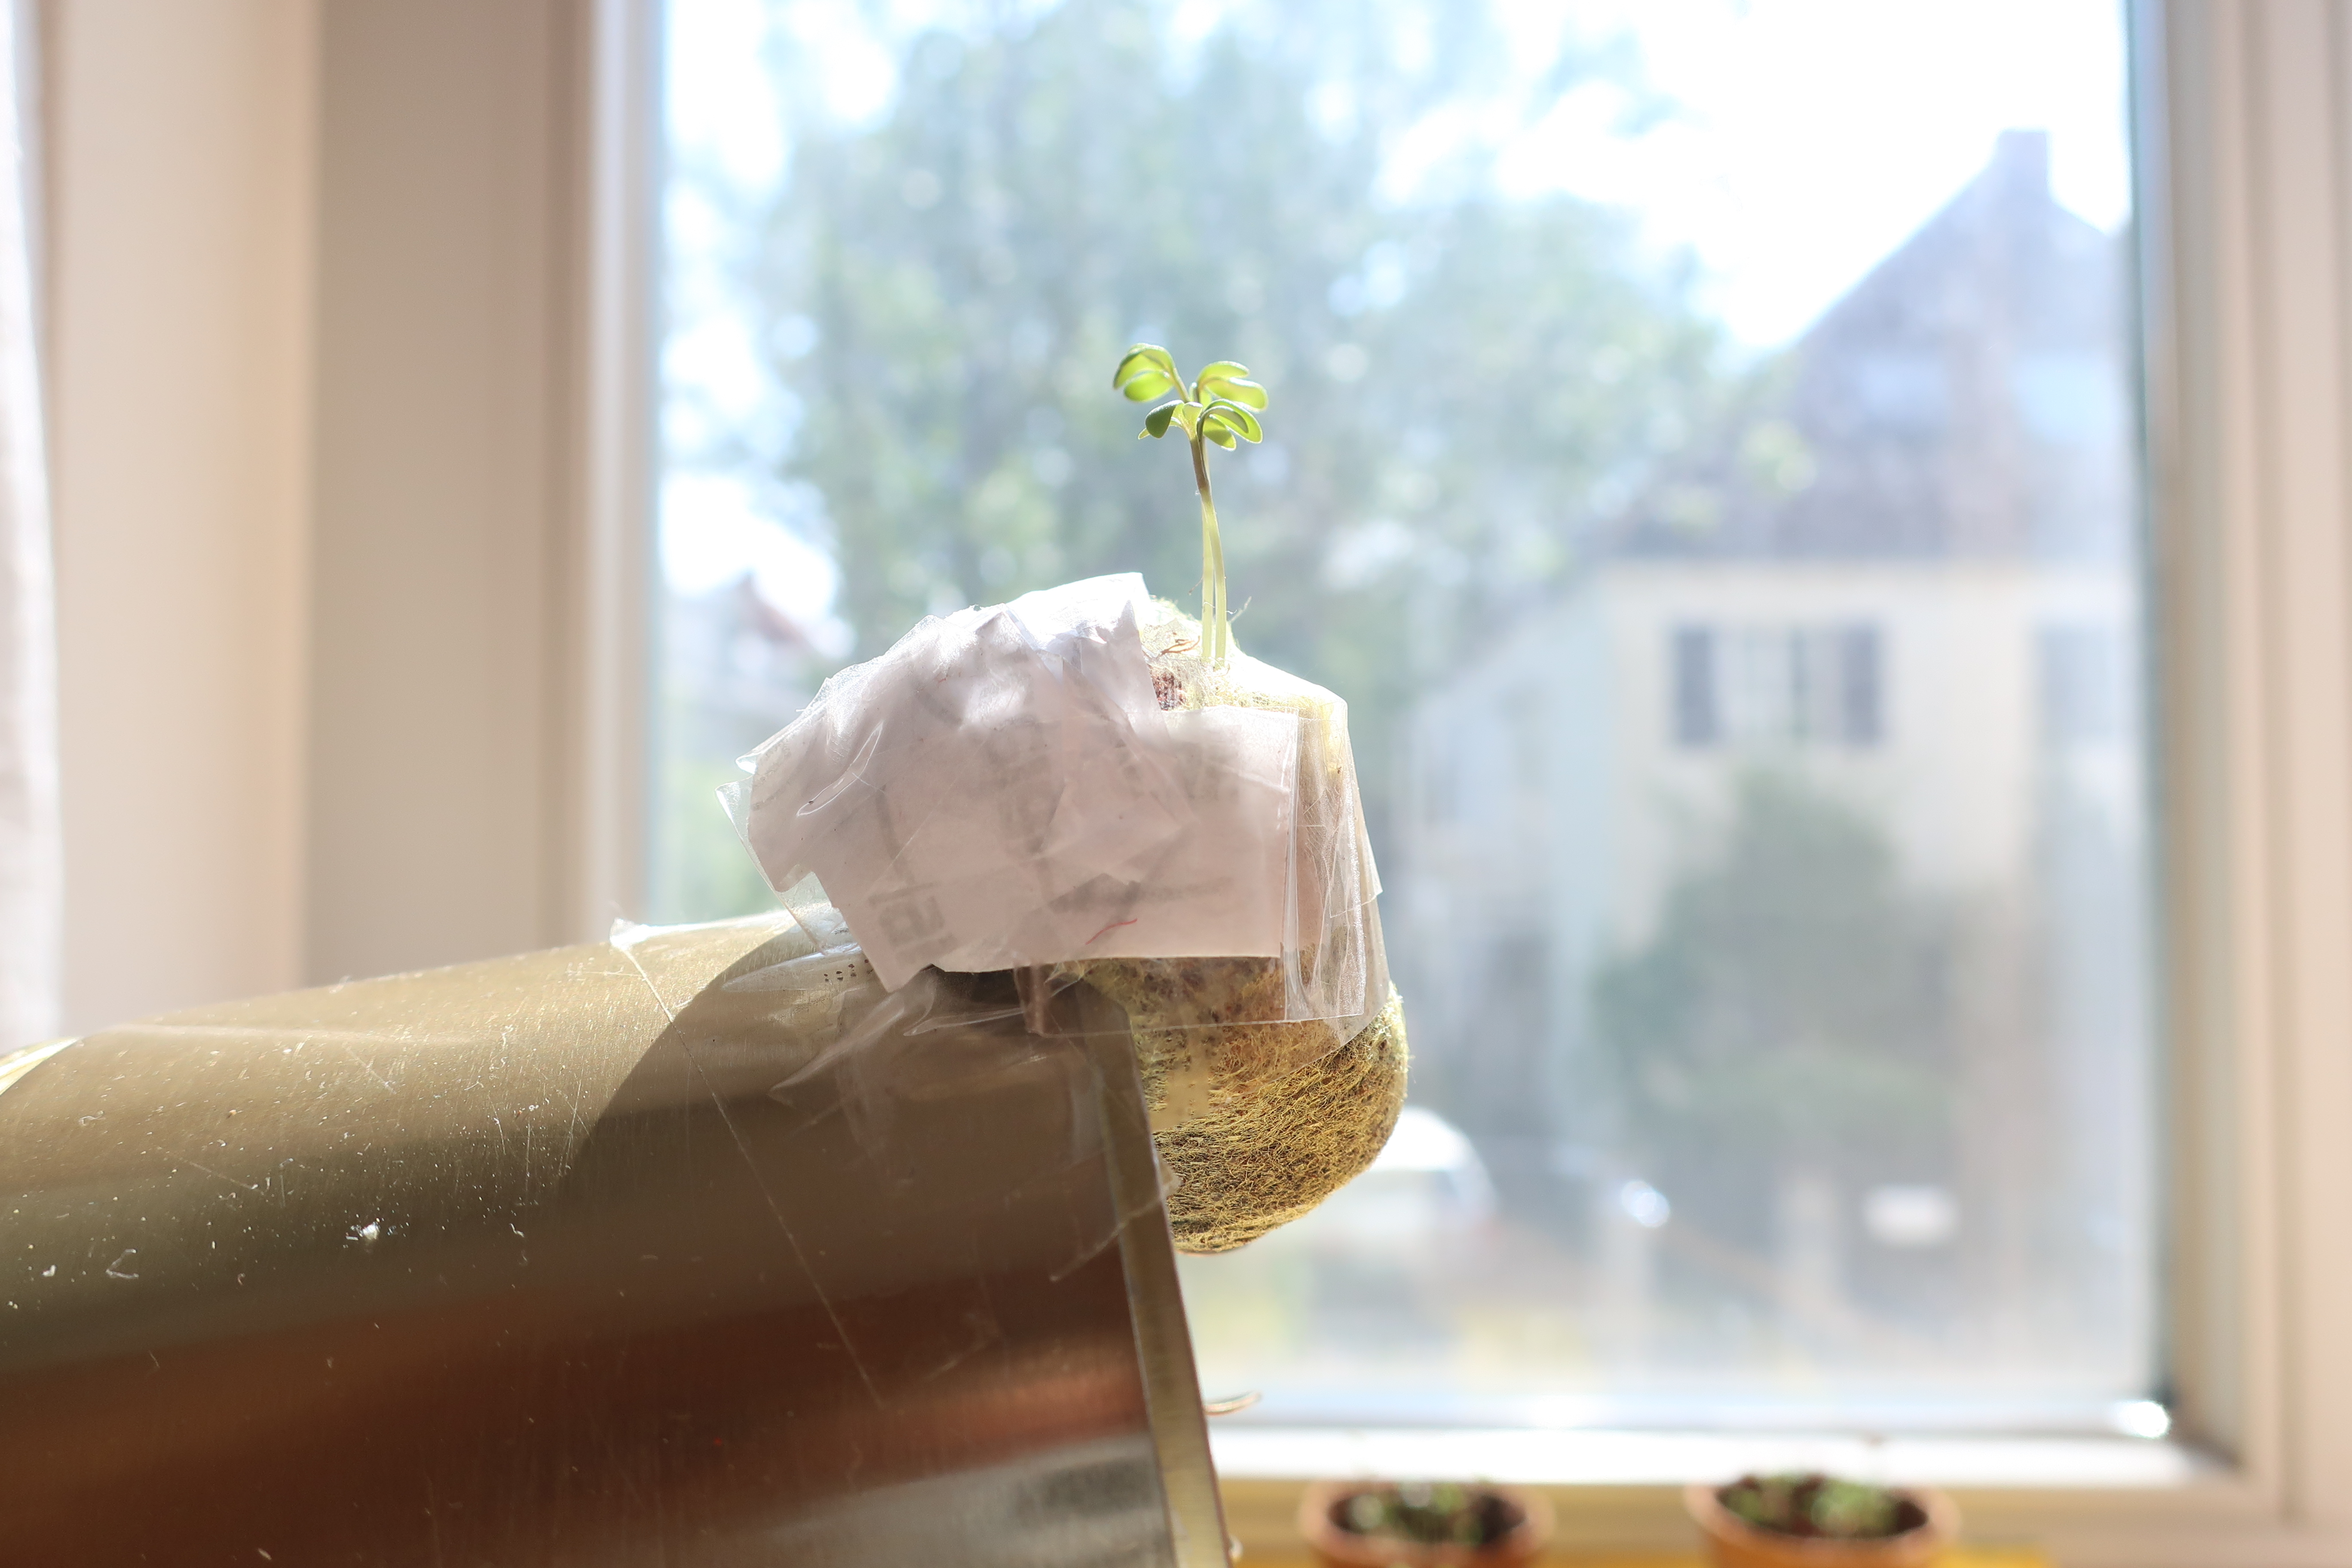
\includegraphics [width = .5\linewidth]{images/IMG_1083.JPG}
%  \end {figure} 
% Photo 1
%
% \begin{figure}
%  \centuring 
%  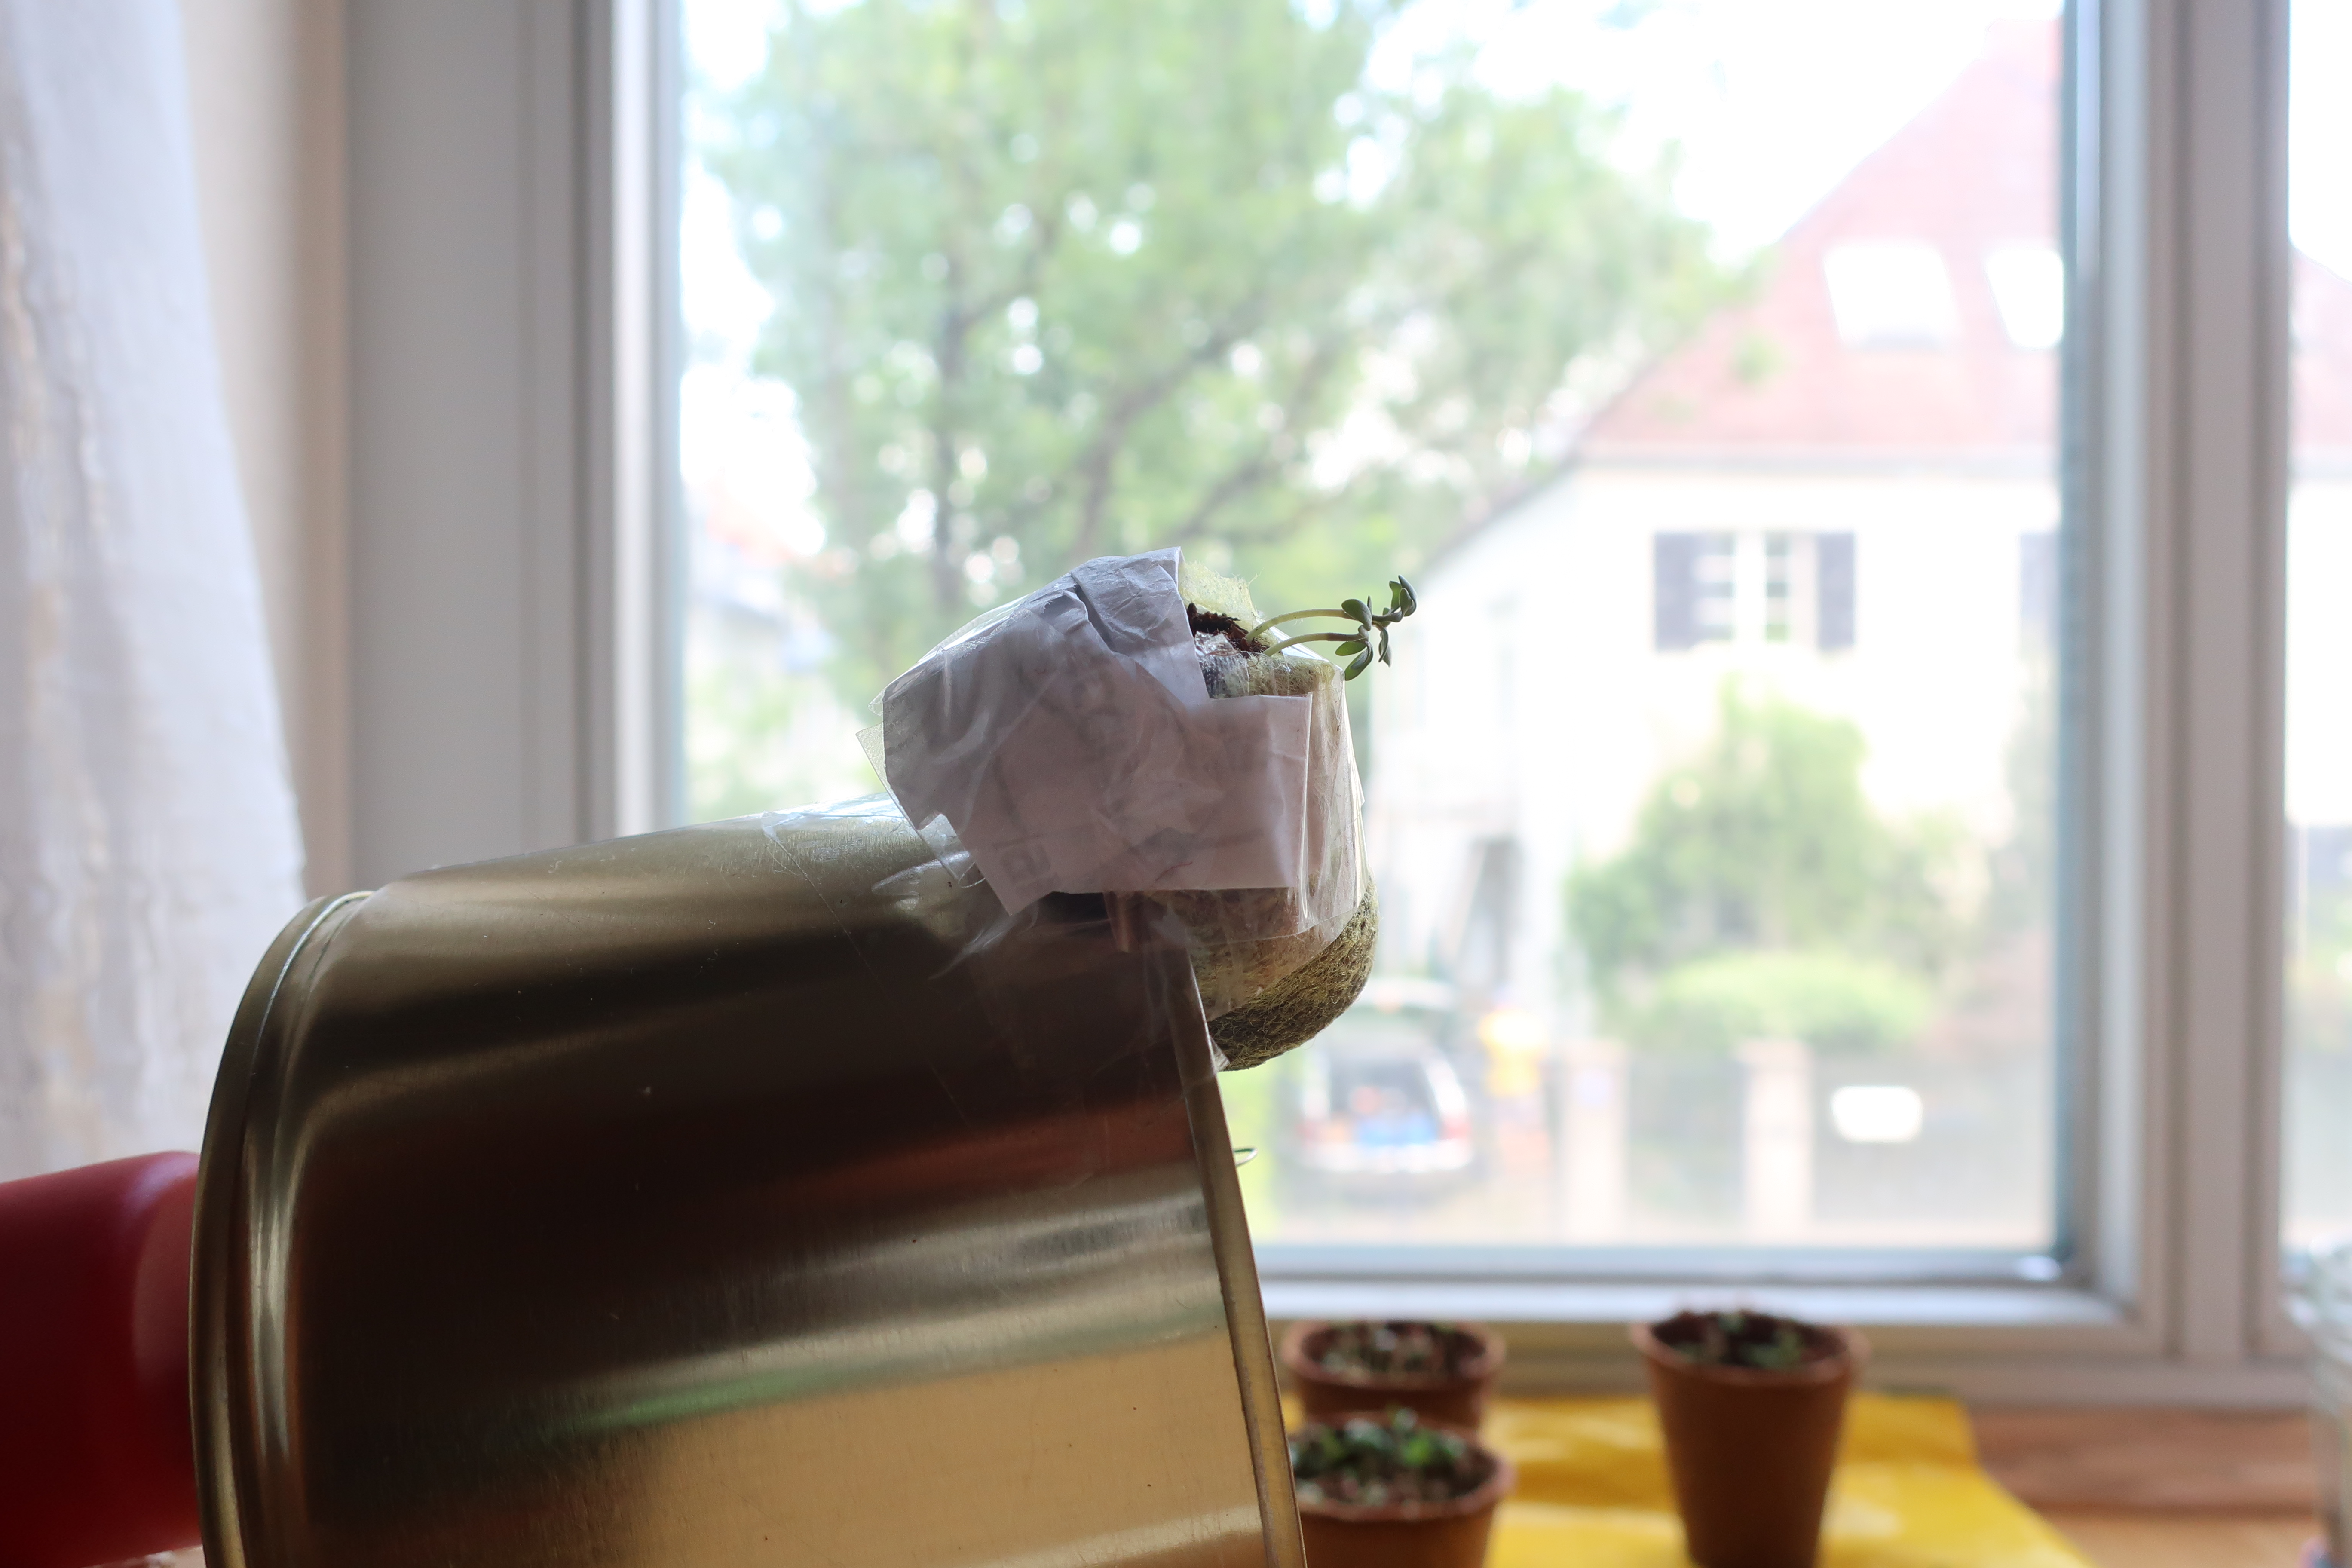
\includegraphics [width = .5\linewidth]{images/IMG_1073.JPG}
%  \end {figure} 
% Photo 2

%\begin{figure}
	%  \centuring 
	%  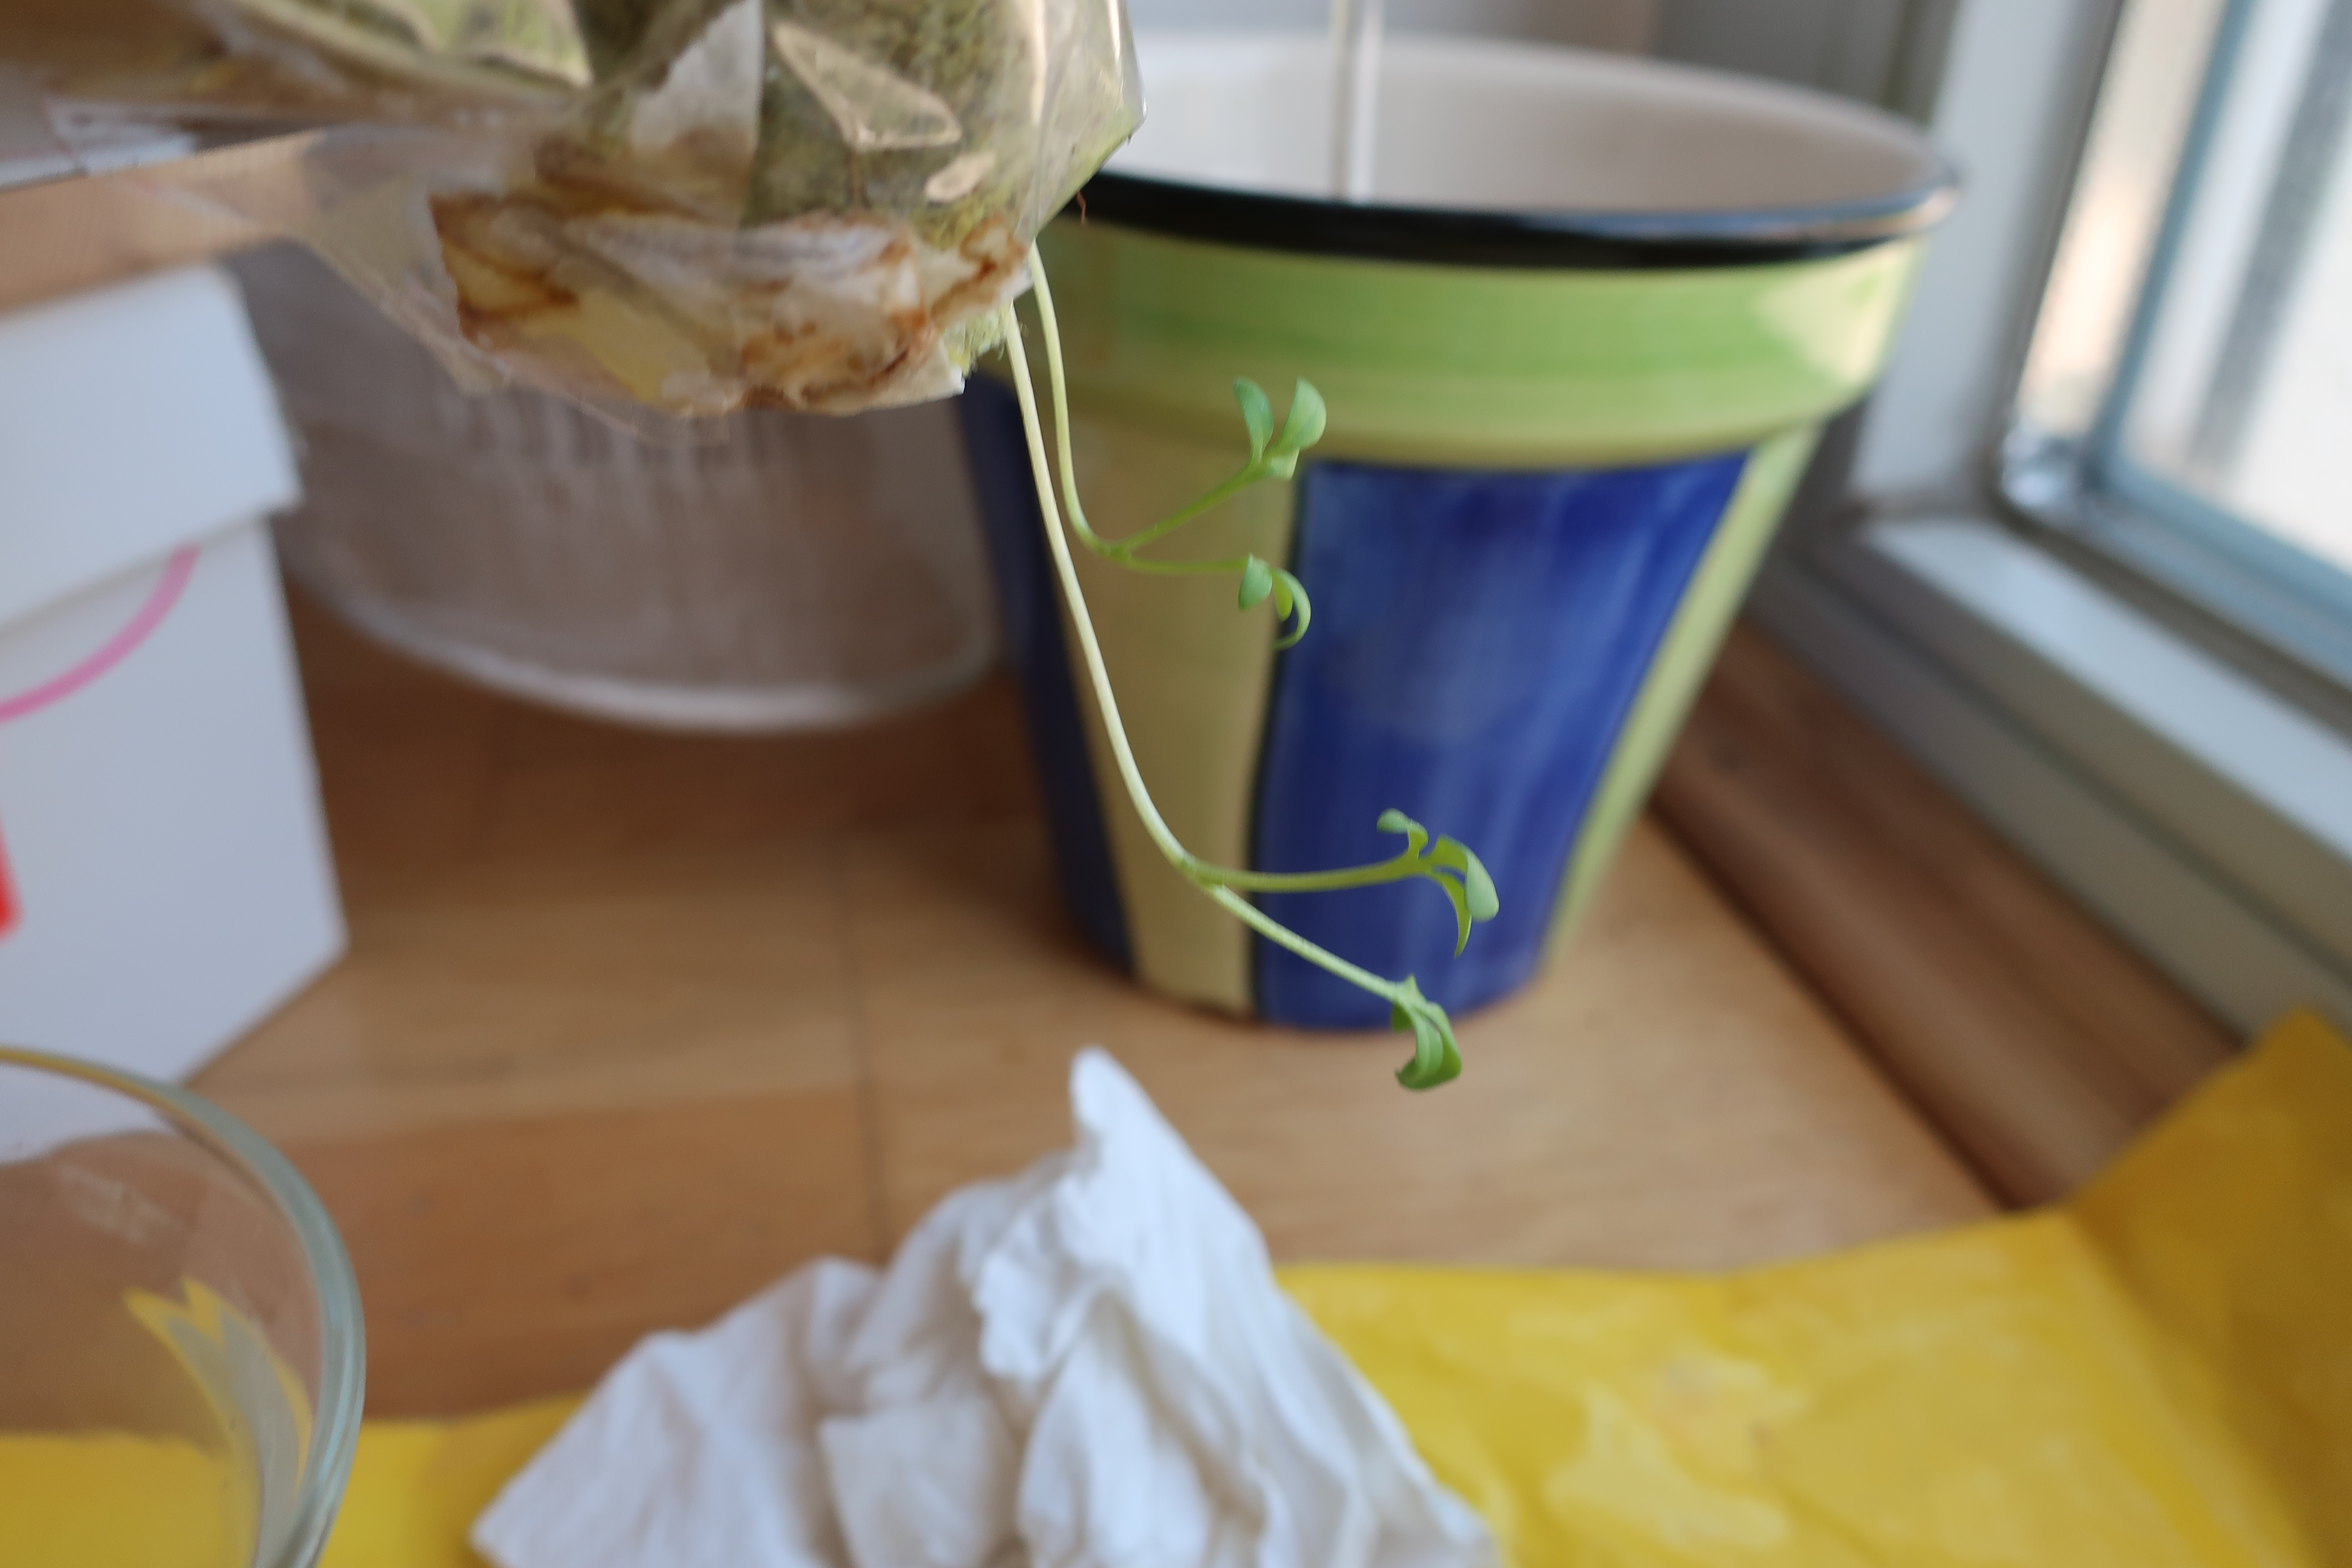
\includegraphics [width =.5\linewidth]{images/IMG_1399.JPG}
	%  \end {figure} 
	% Photo 5

\end{document}
